\documentclass[a4paper,12pt]{article}
\usepackage{graphicx}
\usepackage{caption}

\begin{document}

\section*{Visualisierung der Anfängerzahlen in Informatikstudiengängen}

\subsection*{Grafik 1: Standardposition der Legende}
\begin{figure}[h!]
    \centering
    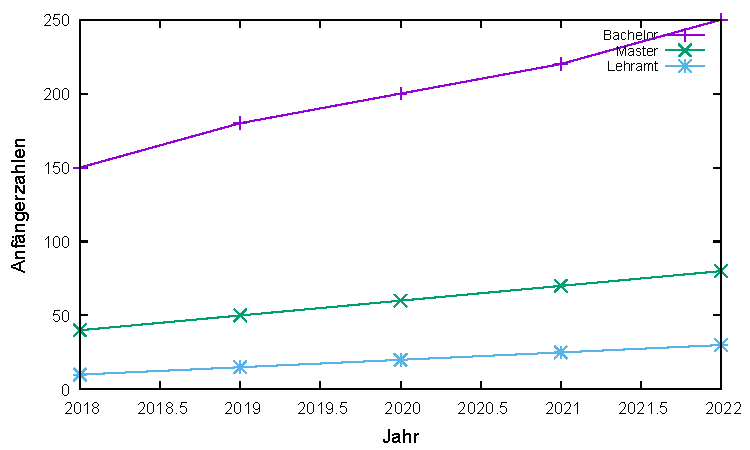
\includegraphics[width=0.8\textwidth]{plot1.pdf}
    \caption{Anfängerzahlen der Informatikstudiengänge (Legende oben rechts).}
\end{figure}

\subsection*{Grafik 2: Legende unten}
\begin{figure}[h!]
    \centering
    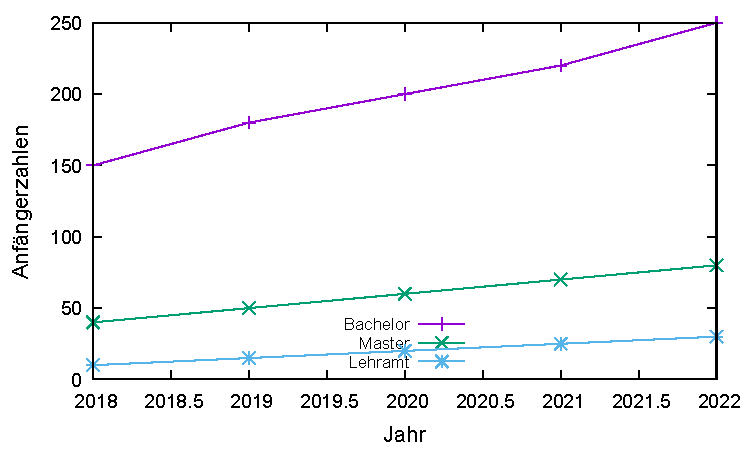
\includegraphics[width=0.8\textwidth]{plot2.pdf}
    \caption{Anfängerzahlen der Informatikstudiengänge (Legende unten zentriert).}
\end{figure}

\subsection*{Grafik 3: Legende links}
\begin{figure}[h!]
    \centering
    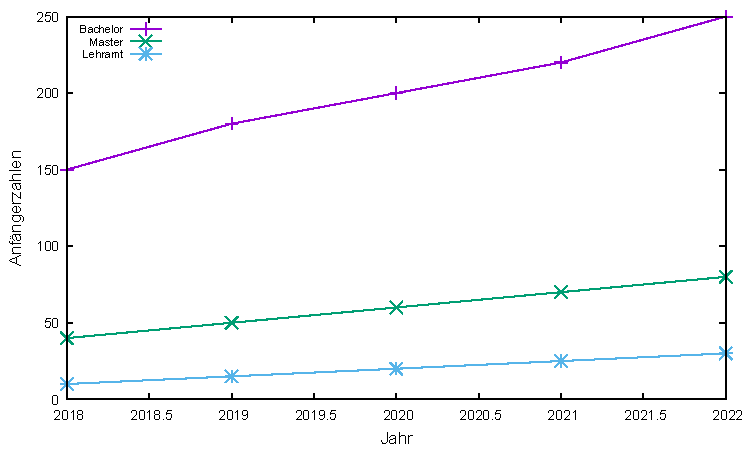
\includegraphics[width=0.8\textwidth]{plot3.pdf}
    \caption{Anfängerzahlen der Informatikstudiengänge (Legende links).}
\end{figure}

\subsection*{Grafik 4: Legende außerhalb des Plots}
\begin{figure}[h!]
    \centering
    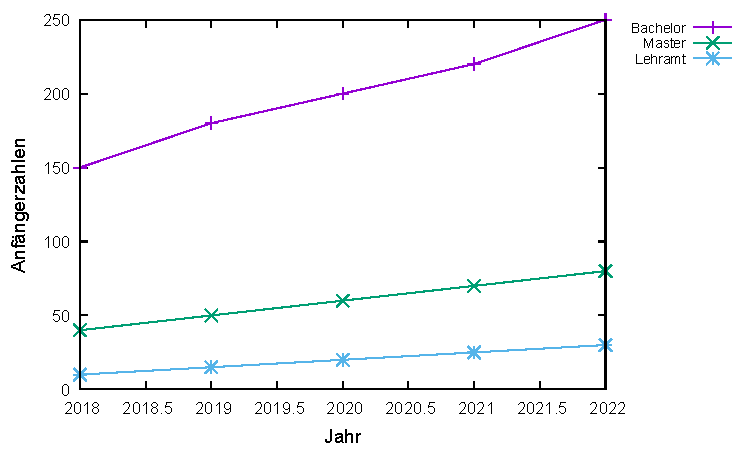
\includegraphics[width=0.8\textwidth]{plot4.pdf}
    \caption{Anfängerzahlen der Informatikstudiengänge (Legende außerhalb).}
\end{figure}

\end{document}
